% =================
% Ghoa
% =================
\subsection{Ghoa}

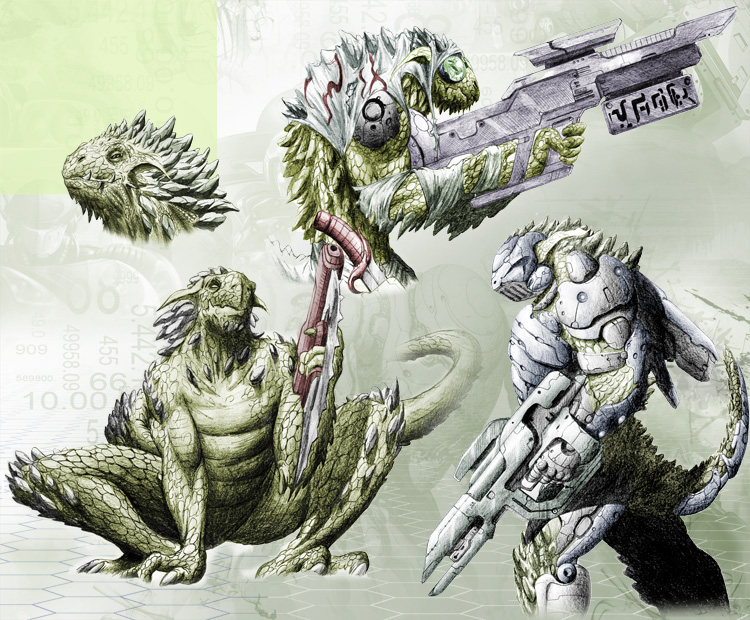
\includegraphics[width=\linewidth]{alien_reptile_concept_by_xjager513-d3ba4g7.jpg}

\begin{redtable}{\linewidth}{sb}
  \textbf{Height} & 170-220cm\\
  \textbf{Weight} & 70-130kg\\
  \textbf{Gender Ratio} & 100\% Hermaphrodite\\
  \textbf{Reproduction} & Viviparity (Live birth)\\
  \textbf{Diet} & Omnivore (meat preference)\\
  \textbf{Homeworld} & (\textit{Unknown})\\
\end{redtable}

The Ghoa (\textit{plural: Ghoan}) are an alien species evolved from an unusual mammal-reptile hybrid native to their homeworld. Their homeworld has been lost to time as the Ghoa place little value on sentimental ties and recorded histories. They are larger and heavier than humans, with sharp ridged scales covering their back. They also have sharp claws and teeth, and have been known to use their tail as a weapon.

The Ghoa are typically tribal, putting their tribe ahead of all other social groups (including the species as a whole). Their chief mode of expression is anger, and the Ghoa are prone to acts of wanton violence. Disputes are traditionally resolved through force, but rarely to the death. Some Ghoa actively embrace the honour and glory of death in battle, and actively seek out combat as mercenaries and pirates.

All Ghoa are hermaphrodites, meaning they have both male and female genitals. Pregnancy is an undesirable period for any Ghoa (as it makes you weaker and more vulnerable during combat), so "females" are usually the Ghoa who are incapable of fighting and have been forced to be subservient to other Ghoa (usually the whole tribe). "Females", or "Breeders", are constantly pregnant in order to produce many warriors for the tribe.

Ghoan characters have the following traits:
\begin{standardtable}{\linewidth}{sb}
  \textbf{Bloodthirsty} & Ghoa are cruel to their foes, rarely take prisoners, and feel little compunction about punishing captured enemies. This causes a -4 Charisma penalty when dealing with "civilised" worlds that know of the Ghoa.\\
  \textbf{Natural Weapons} & The Ghoa use their tails, claws and teeth as weapons, dealing Str+d6 damage.\\
  \textbf{Reptile Blood} & Your prefer warm environments. -4 penalty to resist negative Cold environmental effects\\
  \textbf{Stronger} & Ghoa are stronger than other races. Start with a d6 in Strength instead of a d4.\\
  \textbf{Free Edge} & (Wild cards only) Start with one free Novice Edge\\
\end{standardtable}

\textbf{Ghoan Names}: Bonmok, Chardo, Drothax, Druthak, Dunmom, Garuga, Grintaz, Krudrar, Lakuq, Lugrub, Mugarod, Okrih, Pok, Rok, Roslarb, Sabub, Shak, Shopurd, Trougha, Zugorim

\textbf{Secondary Names}: Ghoa use their tribe as a secondary name. Tribal names are usually descriptive, grandiose, or violent. Tribes are extremely fluid, as new ones are created all the time and do not need to be limited to the Ghoa only (some Ghoa see their teammates as part of their "tribe" and will take on the spacecraft name).
